\documentclass[a4paper,twoside,11pt]{article}
\usepackage[utf8]{inputenc}
\usepackage[english]{babel}
\usepackage{graphicx}
\usepackage{url}
\usepackage{hyperref}
\usepackage{adjustbox}

% pdflatex

% redefinição das margens das páginas
\setlength{\textheight}{24.00cm}
\setlength{\textwidth}{15.50cm}
\setlength{\topmargin}{0.35cm}
\setlength{\headheight}{0cm}
\setlength{\headsep}{0cm}
\setlength{\oddsidemargin}{0.25cm}
\setlength{\evensidemargin}{0.25cm}

\begin{document}

\begin{titlepage}
\begin{center}

% Logo
\resizebox{80mm}{!}{
\includegraphics{../img/logoISEL}}

\vspace{1cm}

% Title
{\Large \textbf{Project and Seminar}\\}
\vspace{0.3cm}
{\Large 2024/2025 - 2nd Semester\\}
\vspace{0.8cm}
{\Large Bachelor in Computer Engineering and Informatics\\}
\vspace{1cm}
{\Huge \textbf{Database Documentation}\\}
\vspace{2cm}

% Authors
\begin{tabular}{c}
    Ângelo Azevedo, n.º 50565, e-mail: \href{mailto:a50565@alunos.isel.pt}{a50565@alunos.isel.pt}\\
    António Alves, n.º 50539, e-mail: \href{mailto:a50539@alunos.isel.pt}{a50539@alunos.isel.pt}\\
\end{tabular}

\vspace{2cm}

% Supervisors
\begin{tabular}{ll}
    {Advisor:} & Pedro Matutino, e-mail: \href{mailto:pedro.miguens@isel.pt}{pedro.miguens@isel.pt} \\
    %  & Alberto Caeiro, e-mail: ac@pc.com, PersonCompany\\
\end{tabular}

\vspace{1cm}

March 2025

\end{center}
\end{titlepage}

\section*{Introduction}
This document provides an overview of the database, entities, attributes, and relationships. 
It also includes implementation decisions.

\section*{Database overview}
The database has been modeled using an Entity-Relationship (ER) approach.
This approach allows for a better understanding of the relationships between entities. The following section shows a figure with the ER model.

The database is implemented with PostgreSQL and tested using fake information in a Docker container.

The following section will address the ER model.
\section*{Entity-Relationship Model}
\begin{figure}[htbp]
	\centering
	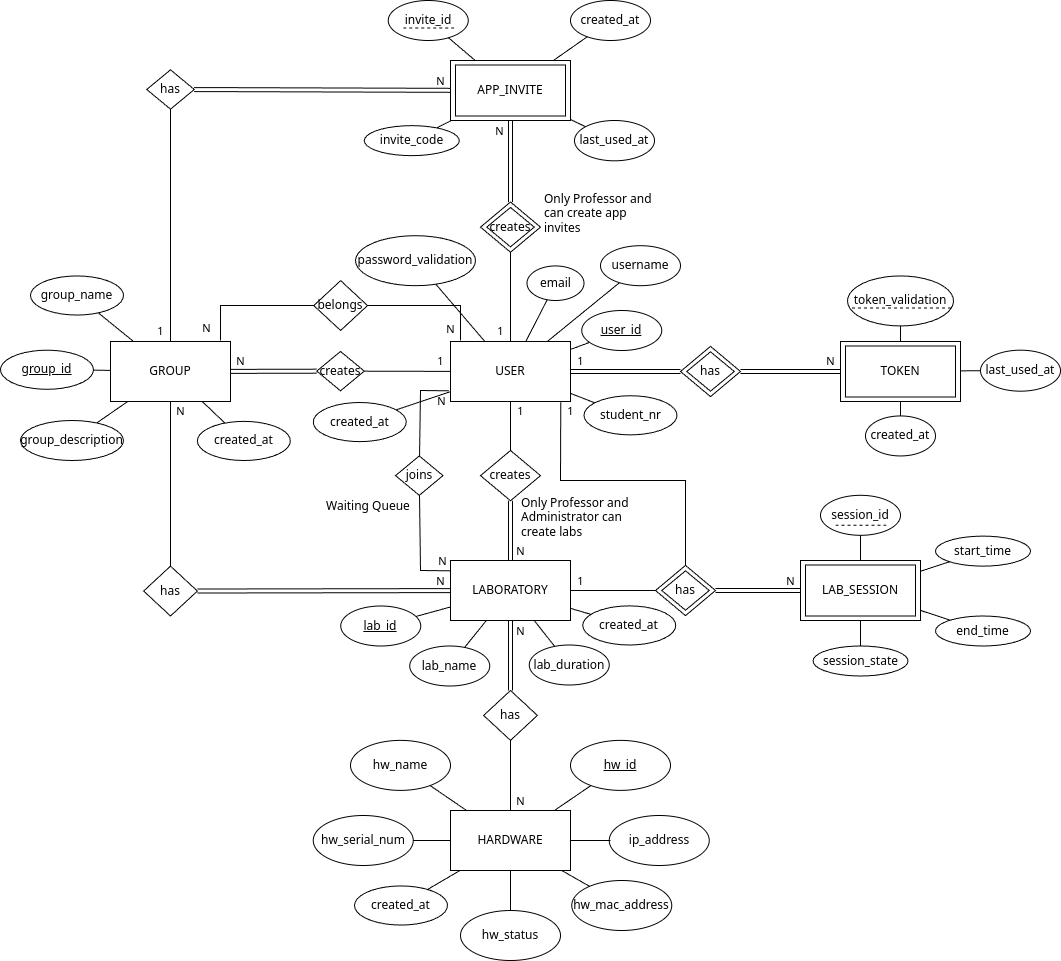
\includegraphics[width=\textwidth]{../img/ERDiagramRL.drawio}
	\caption{Entity-Relationship Model}
	\label{fig:ERModel}
\end{figure}

\section*{Entities and Attributes}
This section provides a comprehensive description of each entity and their attributes.
\subsection*{User}
The first important entity is the \textbf{User}. This entity represents a user in the database.

It has an \textbf{user\_id} as primary key and identity column. An identity column is a special column that is generated automatically from an implicit sequence.
So, whenever a user is inserted in the database it will generate an id. The user\_id is an int data type. This attribute is used to simplify all type of queries made to the database, so that it is only needed a simple number instead of email or username for example. 

It also has, as a char sequence, \textbf{username}, \textbf{email}, and \textbf{password\_validation}. All of them are not null and email is unique. The password\_validation attribute stores the hash of the user's password.
The username attribute, is initially automatically given when a user creates an account. Initially is the same as the email. After the registration, the user can change it to a more specific username. The username should only be used for presentation proposes, since
it is not used to search for a user and can be equal to another user. The email can be used to search for a user since it is unique. The limitations of these attributes are decided by the application domain.

Finally, it has a \textbf{student\_nr} (student number) as an int type and unique and \textbf{created\_at} as a timestamp type and not null.
The student number can be null. This allows users, like professors or others, to be a user entity in the DB. It is worth mentioning that there is not a discriminator attribute because 
this distinction will be implemented in the Role-Based Access Control (RBAC) system.

\subsection*{Token}
\textbf{Token} is a weak entity because it cannot be uniquely identified by its attributes alone. This means that a token needs a user\_id to be identified. This way, a token requires the user to exist.
A token is used for authentication proposes. A user must have a token associated when interacting with the system. 

Since it is a weak entity, it must have a partial key. This partial key is \textbf{token\_validation}. The token\_validation attribute is a randomly hash generated by the system and is used to verify if the user's token is valid, comparing it with this attribute. 
For example, in a scenario where the user token is passed in an authorization header, every time the user makes some interaction, that value should be compared with the value in database. It is a char sequence and not null.

The last attributes are \textbf{created\_at} and \textbf{last\_used\_at}. Both are timestamp types and not null. These attributes are used to check if the token is valid or not. The validation is made by the system and the validation time is decided by the domain.

\subsection*{App Invite}
\textbf{App Invite} is a weak entity. For the same reason as the token, this entity requires the user to exist and cannot be uniquely identified. For example, an app invite should not exist if the user is deleted. An app invite, as the name suggests, is used to invite a user to the system.
A user to register in the system needs an app invite. 

As a partial key, the \textbf{invite\_id} with user\_id uniquely identifies an app invite. This invite\_id is always generated as identity and is an int type. This attribute makes it simple to identify and make queries, with user\_id, an app invite.  

It has an \textbf{invite\_code} attribute as a char sequence and not null. This invite code can take up to 255 bytes, but the actual length is determined by the application domain. With 255 bytes available, it is possible in the future, increase the actual length in the application domain to 255 bytes.

It also has a \textbf{created\_at} and \textbf{last\_used\_at} like the token entity. These attributes can identify which app invite is expired and can give statistics information if needed.

\subsection*{Group}
The \textbf{Group} entity represents a group. This group can be a class of students, a work group, a professor's group, etc...

It has a \textbf{group\_id} attribute as primary key and uniquely identifies a group. It is always generated as identity and is an int type as well. This id make it simple to make queries and identify a group.

Also has a \textbf{group\_name} as a char sequence and not null. This attribute represents the group name chosen by the user. It can be changed after group creation. The limitation of the name group are decided by the application domain. 

It has a \textbf{group\_description} as text type. This is an attribute where a user can write something about the group that they like. It can be null and is a text type.
A text type has an unlimited length, so that the user does not have a limit. In practice, it will have a limit decided by the application domain.

Lastly, it has a \textbf{created\_at}. This attribute has the same characteristics as the token's created\_at. This attribute can be used for statistics proposes.

\subsection*{Laboratory}
\textbf{Laboratory}, as the name indicates, represents a laboratory. 

This entity has a \textbf{lab\_id} as primary key. This is the unique identifier and indicates the laboratory identifier. It is always generated as identity and is an int type. This way, is simpler to identify a laboratory in a query.

It has a \textbf{lab\_name} attribute to represent the laboratory name. It is a char sequence and not null. The limitations are decided by the application domain.

Finally, it has a \textbf{lab\_duration} attribute to represent the duration of each lab session, in \textbf{minutes}. It is an int type, is not null.
And it has a \textbf{created\_at} attribute similar to the group's created\_at.

\subsection*{Lab Session}
The \textbf{Lab Session} is a weak entity. This session should only exist if associated with a user and a laboratory. It represents a lab session, that is, a session where a user can manipulate something in the laboratory.

As attributes, it has \textbf{session\_id} as a partial key. With user id and lab id, a lab session can be uniquely identified. It is always generated as identity and is an int type. This way, is simpler to identify a session in a query.

It has \textbf{start\_time} and \textbf{end\_time} attributes to represent the date and hour when a session starts and ends. Both are timestamps and not null.

Lastly, it has a \textbf{state} attribute to indicate the session state, that is, if it is active, inactive, or scheduled. This attribute is a char sequence and is not null. If necessary, additional states can be defined for this attribute. If more states are added, this document should be updated.

\subsection*{Hardware}
The last entity is \textbf{Hardware}. This entity can represent any hardware. For example, it can represent a computer or an FPGA.

As primary key, it has a \textbf{hw\_id}. It is always generated as identity and is an int type. This attribute uniquely identifies the hardware. This way, is simpler to identify a hardware in a query.

It has a \textbf{hw\_name} attribute for the hardware name. It is a char sequence and not null. 

It has a \textbf{hw\_serial\_num} attribute that represents the hardware serial number. It is a char sequence and not null. 

It also has an \textbf{ip\_address} and \textbf{hw\_mac\_address}. Both are char sequences and depending on the type of hardware, these attributes can be null.

It has a \textbf{hw\_status} attribute as a char sequence and not null. This attribute indicates the status of the hardware, such as available, occupied, etc.

Finally, it has a \textbf{created\_at} attribute with the same characteristics as the laboratory's created\_at.

\section*{Associations}
This section provides a comprehensive overview of the associations between entities. This overview should explain how the system will work.

\textbf{User} has associations with:
\begin{itemize}
    \item \textbf{Token} - This must be weak association, as explained before. A user has a token and this token is created automatically by the system when is needed. A user can have \textbf{N} token but a token has \textbf{only one} user.
                           Because of this, the primary key of the user is in the token's table has primary key with the partial key token validation. 
    \item \textbf{App Invite} - This is a weak association, because of the relationship with the user. A user can create \textbf{N} app invites but a app invite is created \textbf{only by one} user. As the same as the token, the app invite's table will have the primary key of the user.
    \item \textbf{Group} - User has two associations with group:
    \begin{itemize}
        \item The first association is \textbf{creates}. A user can create \textbf{N} groups but a group can only be created \textbf{by one} user.
        \item The last association is \textbf{belongs}. A user can belonge to \textbf{N} groups and a group can have \textbf{N} users.
    \end{itemize}
    \item \textbf{Laboratory} - User has two associations with laboratory:
    \begin{itemize}
        \item The first association is \textbf{creates}. A user can create \textbf{N} laboratories but a laboratory is only created by \textbf{one} user. 
        \item The last association is \textbf{joins}. This association represents a queue to a laboratory. A user can join \textbf{N} laboratories and a laboratory is joined by \textbf{N} users. In practice, this is not true because the app domain is going to have some restrictions, for example, a user cannot join more than one laboratory. But for the database propuses this has to be a relationship \textbf{N} to \textbf{N} so that a user, when finished doing something in a laboratory, can joined other laboratory. Also, this will save the history of the joined laboratories. 
    \end{itemize}
    \item \textbf{Lab Session} - This is the last association. This association is weak and represents the session a user has with a laboratory. A user can have \textbf{N} sessions but a session has only \textbf{one} user.
\end{itemize}

\textbf{App Invite} has only one more association. This association is with group entity. This associations represents the connection a app invite has with a group. This allows that an app invite has a association with a group so that, when used by a user when registering, to be associated immediately.
An app invite has only \textbf{one} group associated but a group can be associated with \textbf{N} app invites.

\textbf{Group} also has only one more association. Has a association with laboratory representing wich group can enter a laboratory. Only users in the group can join the laboratory. A group is associated with \textbf{N} laboratories and \textbf{N} laboratories are associated with \textbf{N} groups.

\textbf{Laboratory} has the following associations:
\begin{itemize}
    \item \textbf{Lab Session} - This association indicates wich laboratory a session is. A laboratory has \textbf{N} sessions but a session is only associated with \textbf{one} laboratory.
    \item \textbf{Hardware} - The last association is with hardware. This association represents the hardware that is assigned with a laboratory. A laboratory can have \textbf{N} hardware and a hardware can be assigned to \textbf{N} laboratories.
\end{itemize}

This concludes the associations between entities. Worth mentioning that some restrictions are not mentioned here because is part of the web api. To learn more about some restrictions check the web api documentation. 

\nocite{*}
\bibliographystyle{plain}
\bibliography{references}

\end{document}